\documentclass{article}
\usepackage{graphics} 
\usepackage{graphicx}

%% Key definitions for text elements. USE THEM
\def\secref#1{Sec.~\ref{#1}}
\def\figref#1{Fig.~\ref{#1}}
\def\tabref#1{Tab.~\ref{#1}}
\def\eqref#1{Eq.~(\ref{#1})}
\def\algref#1{Alg.~\ref{#1}}
\def\appref#1{App.~\ref{#1}}

\newcommand\etal{\emph{et al.}}

\title{\LARGE \bf Semantic Perception, Mapping and Exploration}

\begin{document}
	
	\maketitle	
	
	\section*{Introduction}
	
	\section*{Related Work}
	
	Acquisition and modeling of semantic information is a key requisite for mobile robots to be deployed in human environments. In this field, fundamental aspects faced by research are: the recognition of places and objects, the construction of semantic models and the exploration strategies to enrich contextual knowledge. In the remainder of this section, we will present relevant work that focused on the mentioned problems, namely: semantic perception, semantic mapping and semantic exploration.
	
	\subsection*{Semantic Perception}
	Extracting semantic information from visual data is one of the  fundamental problems of computer vision. Scene understanding can be decomposed into sub-tasks, depending on the information one is interested to extract from the input data. These sub-tasks can be organized on a progression that goes from coarse to fine grained inference.
	
	Image classification is the task of assigning a semantic label to an input image from a fixed set of categories. Ulrich and Nourbakhsh \cite{ulrich2000icra} propose an appearance-based place recognition system for topological localization. They use colour histogram features \cite{swain1991ijcv} and a simple voting scheme for nearest-neighbor matching. In a similar fashion, Torralba \etal~\cite{torralba2003context} derive an hidden Markov model (HMM) for place recognition and new place categorisation based on the global statistic feature retrieved from texture \cite{oliva2001ijcv}. In contrast, Lisin \etal~\cite{lisin2005cvpr} propose to model classes of images as a probability distribution over local features, in order to be combined with global features. This method has proven to perform well in applications where a rough segmentation of objects is available.
	
	Object detection consists of making a prediction not only of object categories but also of their spatial locations. A seminal work can be considered that of Viola and Jones \cite{viola2004ijcv}, who proposed a fast and robust face detection. Their method makes use of Haar-like features \cite{papageorgiou1998iccv} to search for likely face candidates, which can then be refined using a cascade of more expensive but selective detection algorithms \cite{freund1997jcss}. Likewise, a well-known example of pedestrian detection has been proposed by Dalal and Triggs \cite{dalal2005cvpr}, who use a set of overlapping Histogram of Oriented Gradients (HOG) descriptors fed into a Support Vector Machine (SVM) \cite{cortes1995support}.
	
	Image segmentation is the task of finding groups of pixels that possess some "similarity" and is one of the oldest and most widely studied problems in computer vision.
	Early techniques focus on local region merging and splitting \cite{ohlander1978picture,brice1970scene}, while, more recent algorithms often optimize some global criterion, such as intra-region consistency and inter-region boundary lengths or dissimilarity \cite{comaniciu2002pami,shi2000pami,felzenszwalb2004ijcv,chan2001ip,osher1988jcp}. 
	
	Despite the popularity of the presented methods, a recent breakthrough in scene understanding has been the adoption of Convolutional Neural Networks (CNNs) \cite{garcia2017review}. Krizhevsky \etal in \cite{krizhevsky2012nipsjournal} present the pioneering deep CNN that, despite its simplicity, won the Imagenet 2012 classification challenge with wide margin on the closest competitor. Similarly, different object detection methods based on deep neural netowrks have shown to outperform the state-of-the-art \cite{redmon2016cvpr,erhan2014cvpr,liu2016eccv}. Consequently, the capabilities of such networks have been also investigated in pixel-level labeling problems like semantic segmentation. In this context, a milestone is the work of Long \etal~\cite{long2015cvpr} who transformed existing classification models (\cite{simonyan2014very,szegedy2015cvpr}) into fully convolutional ones to output spatial maps instead of classification scores. One of the main reason behind its popularity is that, with this approach, CNNs can be trained end-to-end and efficiently learn to make dense predictions with inputs of arbitrary size.
	
	\subsection*{Semantic Mapping}
	
	Building a digital representation of the environment where the robot has to operate, is a well studied problem in both robotics and AI communities (citations needed). In literature,  different types of representations have been proposed, as well as different methods to obtain each of them. It  is possible to classify these representations by the type of information they convey to the robot, i.e.: metric, that can be used to measure physical quantities in the environment such as distance to obstacles; topological, that allows the robot to assess the connectivity between places and/or objects in the environment and semantic, that tells the robot to which category the objects in the map belong to. Traditional approaches dealt with the reconstruction of metric and topological information, whereas, recent years have seen growing interest in enriching the existing representations with semantics \cite{kostavelis2015semantic,liu2016extracting}. This involves segmenting a scene by assigning a label to the extracted features and mantaining the correspondence with already seen features to integrate the current measurement in a globally consistent model.
	
	Hermans et al., in \cite{hermans2014dense}, address the problem of dense semantic segmentation of 3d point clouds. Here, the term "dense" indicates that the proposed method works with the whole measurement returned by the sensor, thus, each feature is a single point of the 3d point cloud obtained from the RGB-D camera. In this work, the authors propose a mapping scheme which is made of three components: a Randomized Decision Forest (RDF) to obtain a 2D segmentation of the RGB image, a 3D scene reconstruction to obtain a geometric model of the environment and the correspondence between features of two consecutive frames and, finally, a Conditional Random Field \cite{krahenbuhl2011efficient} to properly assign the semantic labels of the 2d segmentation to the 3d points of the geometric model. A significant contribution of this work is that the proposed pipeline can meet real-time requirements, however, segmentation results are not comparable with offline methods.
	
	McCormac et al. \cite{mccormac2017semanticfusion} follow a similar approach to the one described so far, with the difference that they use a Convolutional Neural Netowork \cite{noh2015learning} to obtain a semantic segmentation of the RGB image.  This clearly improves classification results, as CNNs have shown impressive performance on such tasks, however still it's not clear how a semantically annotated 3d point cloud can be used by the robot for its purposes. This is because a point cloud is an unstructured representation, i.e. no connectivity information is provided, making it not suitable for tasks like path planning and execution.
	
	In (cite), Gunther et al. consider a different model to represent the environment, that is, instead of using a point cloud, which can be seen as a low-level representation, their model is directly made of objects. To build such a model, the authors use a 3d object recognition system, which, given a 3d point cloud, returns the set of objects detected in the scene in terms of their 3d pose, bounding box and semantic label. Moreover they propose an effective segmentation scheme that takes advantage of the contextual relations inherent to human-made spaces in order to improve classification results. This is achieved by building a graph, from the objects in the scene, which is exploited by a CRF to smooth the output of the object recognition. The main drawback of this method, is that the object recognition method guarantees reasonable results only under strong assumptions, that is, the scene observed by the robot must be a table, the objects in the scene must be already known and a CAD model for each of them must be available.
	
	A possible solution to this shortcoming is to keep the map representation proposed in Gunther et al., while using a more sophisticated method to segment the scene. Nowadays, CNNs are proving to be an effective solution for visual problems like that, thus, it's a reasonable idea to consider their use in such a context.
		
	\subsection*{Semantic Exploration}
	
	\section*{Technical Section}
	
%	Our system to build and maintain a semantic map is made of three components: perception, mapping and exploration.
%	
%	\begin{itemize}
%		\item perception: given an RGB-D frame, detects objects
%		\item mapping: builds a local map from the current view and updates the global map
%		\item exploration: finds the best view to improve robot knowledge of the environment
%	\end{itemize}
%	
%	These components communicate with each other exchanging data structures. Perception receives frame from exploration and returns an array of detections. A detection is an entry in a list whose fields are: type, position, size and pixels. Mapping receives detections, builds 3D objects from it (local map), performs data association with global map and merges the two. An object is an entry in a list (map) whose fields are: type, pose, size and model.
	
	Our pipeline is made of three modules that exchange data structures among each other to build and maintain a semantic map. The perception module is in charge of classifying objects seen by the robot, it receives an RGB-D frame from the camera and returns the set of detections. The mapping module builds a local map from the objects detected by the perception module and updates the global map by performing data association and merging. Finally, the exploration module takes as input the updated global map and current robot pose and finds the best view to improve robot knowledge of the environment.
	
	\subsection{Perception}
	
%	Given an image and a set of semantic classes, semantic segmentation is the task of localizing and classifying objects in the view and label each pixel according to its semantic class. How to perform segmentation in a simulated environment. You know the pose of objects and robot in the world. If you assume that the robot is equipped with a sensor that has a known field-of-view, then inferring which object the robot is perceiving requires some geometrical computations. Then, it's necessary to decide which elements of the scene are visible, and which are hidden. This is typically solved with a Z-buffer in Computer Graphics. Since we know that the robot is equipped with a visual sensor, we can assume that the depth image is indeed a Z-buffer, thus, we use this information for occlusions check.
%	
%	Input: set of models, robot pose. Output: set of detections. Steps: for each model, check if it's in frustum and transform it into camera frame. for each pixel of the depth image check if it falls into a model bounding box and assign it to its detection.
	
	Semantic segmentation can be regarded as the task of localizing and classifying objects in the scene and label each image pixel according to its semantic class.
	More formally, given an image I and a set of semantic labels L, semantic segmentation computes an assignment to each image pixel x of a label l.
	
	In a simulated environment it's possible to execute this task by performing geometrical computations. Since we know the pose of the objects and the robot in the world, if we assume that the robot is equipped with a sensor that has a known field-of-view, inferring which objects the robot is perceiving can be done through view frustum culling (cite), as shown in (fig). After this step, it's necessary to decide which elements in the view frustum are visible by the robot, and which are hidden. This is a well-known problem in Computer Graphics and can be solved with a Z-buffer algorithm (cite). Since we know that the robot is equipped with a visual sensor, we can assume that the depth image D is indeed a Z-buffer, thus, we use this information for occlusion check.
	
	\subsection{Mapping}
	
%	Semantic mapping is the task of incrementally updating a semantic map with the current frame. Assuming that the two maps are in the same reference frame, data association is performed to find corresponding objects. Remarks: it's a crucial step, high-level features makes the problem easier.	In case of a limited number of objects, brute-force is a reasonable technique to choose. In the simulated environment, the knowledge of the semantic class is perfect. In real world scenarios, object detectors return a probability distribution over semantic labels. In the first case, the corresponding object is the closest one with the same type. In the second case, euclidean distance could be scaled with class probabilities to represent a form of similarity measure.	Once data association found object correspondences, it's time to perform the actual update of the map. Input: maps, correspondences. Output: updated global map. Steps: for each object in local map check if it's already been seen, yes: merge, no: add to map. This strategy may fail in case of false positives returned by data association. Possible solution:  aging scheme.
%	
	Semantic mapping is the task of incrementally updating a semantic map with incoming frames acquired by the robot. A semantic map is an array of objects, each object is defined by: type, pose, size, model. Objects are extracted from the depth image and assembled in a local map. Then, data association is performed to find corresponding objects between local and global map and update the global map accordingly.
	
	 
    \begin{figure}[htbp]
		\centering
		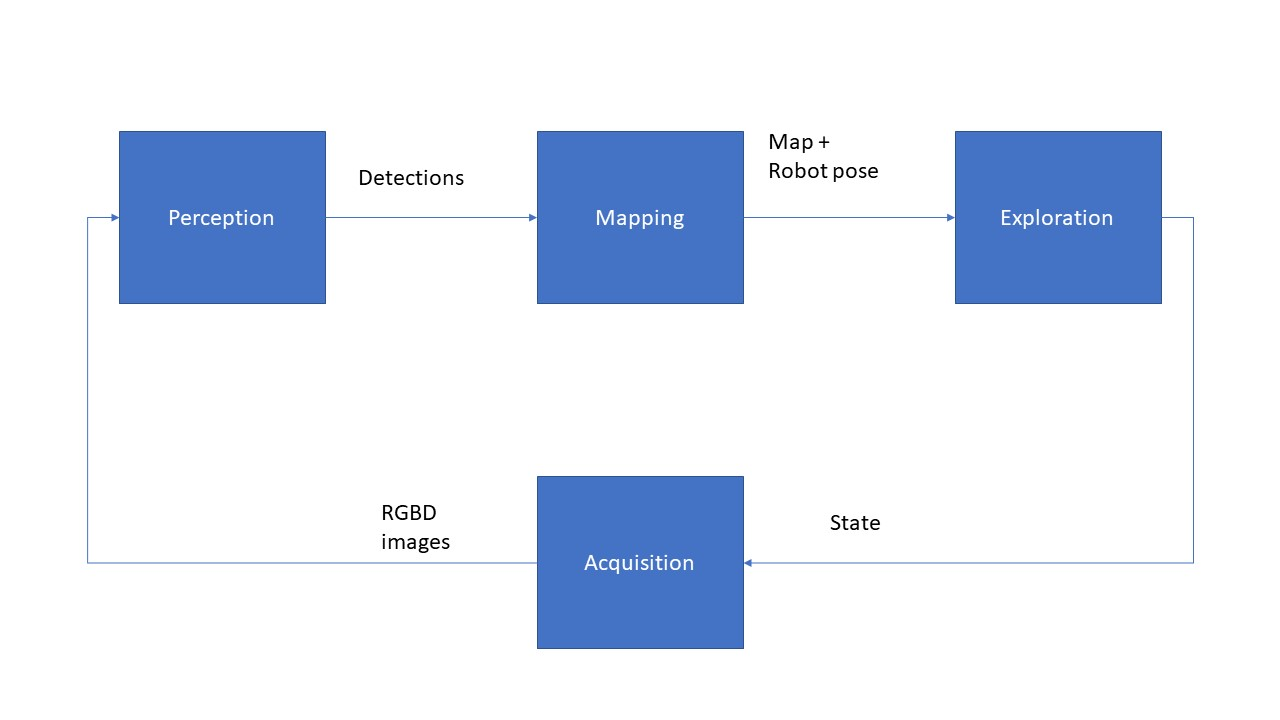
\includegraphics[width=\linewidth]{pics/pipeline}
	\end{figure}	
	
	
	\bibliography{references}
	\bibliographystyle{plain}
	
\end{document}